\section{La gestion de tâches asynchrones}
\begin{figure}[H]
    \centering
    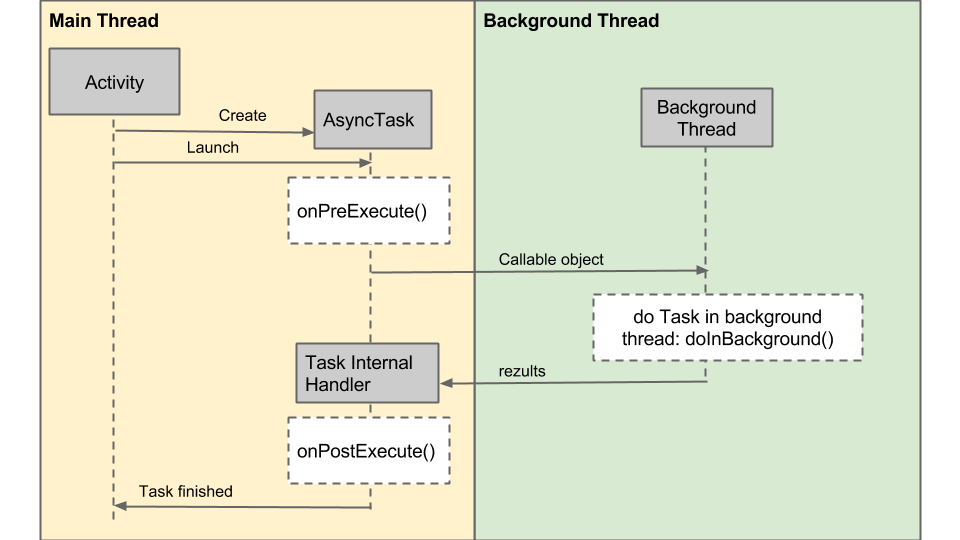
\includegraphics[width=1\textwidth]{assets/asynctask_seqdiagram.png}
    \caption{La classe \code{AsyncTask}}
\end{figure}

\begin{lstlisting}[language=java]
private class DownloadFilesTask extends AsyncTask<URL, Integer, Long> {
    protected Long doInBackground(URL... urls) {
        int count = urls.length;
        long totalSize = 0;
        
        for (int i = 0; i < count; i++) {
            totalSize += Downloader.downloadFile(urls[i]);
            publishProgress((int) ((i / (float) count) * 100));
            
            // Escape early if cancel() is called
            if (isCancelled()) break;
        }
        
        return totalSize;
    }
    
    protected void onProgressUpdate(Integer... progress) {
        setProgressPercent(progress[0]);
    }
    
    protected void onPostExecute(Long result) {
        // Note: pas bien, il faudrait associer un écouteur
        // et passer directement le message.
        showDialog("Downloaded " + result + " bytes");
    }
}

new DownloadFilesTask().execute(url1, url2, url3);
\end{lstlisting}
